\section{Marco Teórico}

\begin{figure}[ht!]
   \centering
   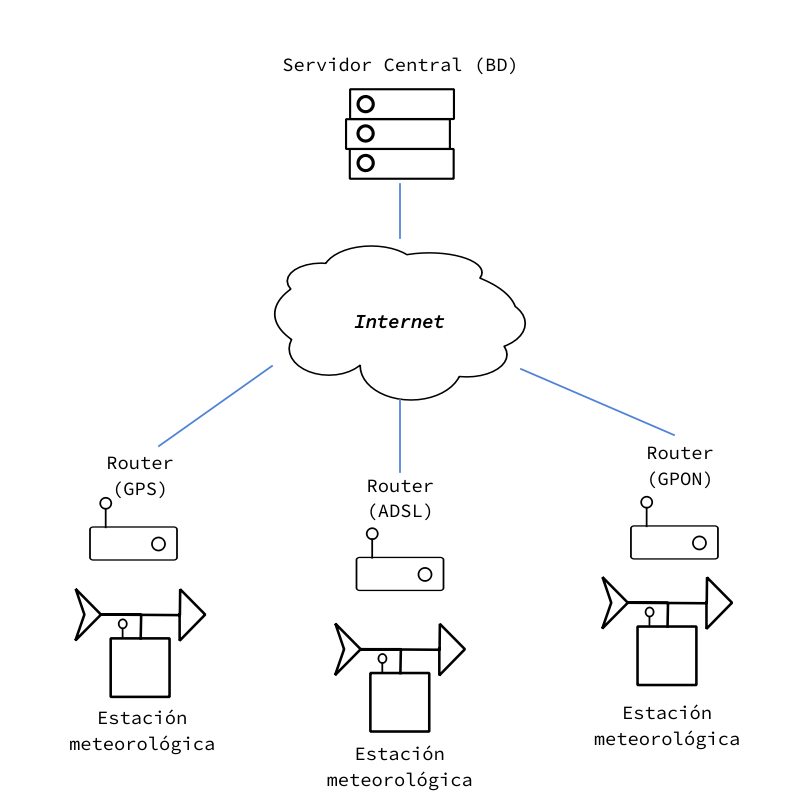
\includegraphics [ width = 0.8\textwidth ] {images/stations_arrangement.png}
   % 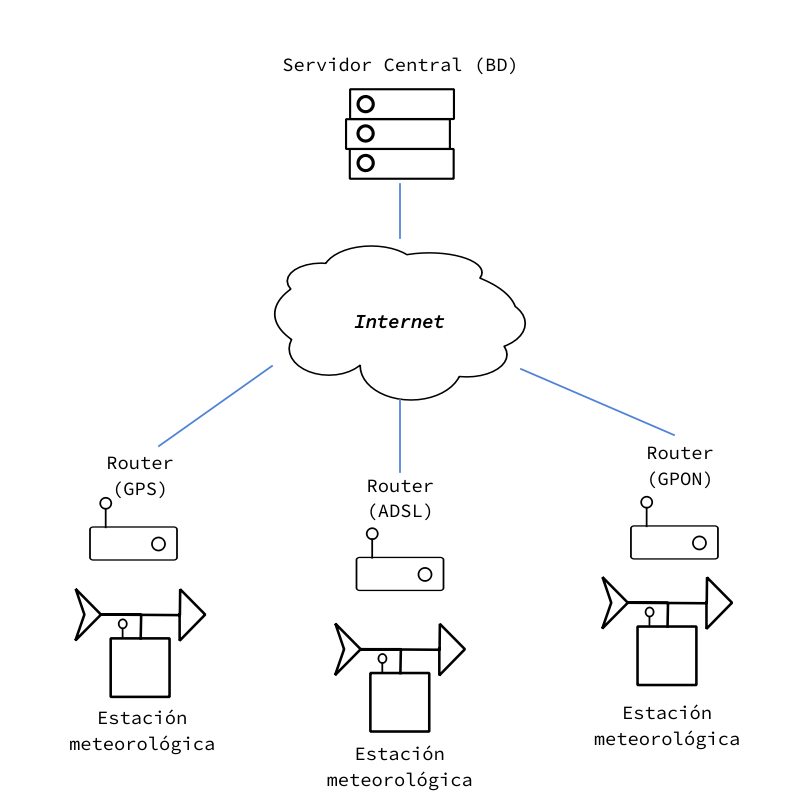
\includegraphics [ height = 160px ] {images/stations_arrangement.png}
   \caption{Organización de las estaciones meteorológicas en el laboratorio CECATEV}
   \label {fig:stations}
\end{figure}

Transformadas de Fourier

$\mathscr{L}\{f(t)\}=F(s)$

Climatología
   Presión barométrica
   Temperatura
   Velocidad del viento
   Dependencia de variables climatológicas

Meteorología
   Normalización de Temperatura
   Estacion meteorológica

   % NOAA

Sensores


\subsection{Métodos de compresión}

La compresión de datos se realiza por medio de diversas

   Ruido
      Reducción de ruido
      Normalización de temperatura por medio de Filtros
   Fourier

% ¿Es válido confiar en el spreadsheet de la empresa que vende los elementos? SI. NO ES DE INSTRUMENTACIÓN LA TESIS
Tiempo de actualizacion de datos, por variables fisicas.
\cite{davis:6152C_6162C_SS}.

% ¿Es realmente factible codificar los datos en una RaspberryPi? ¿Se utiliza el GPU o que pedo?

